\documentclass{article}

\usepackage[spanish]{babel}
\usepackage{wrapfig}
\usepackage{amsmath}
\usepackage{graphicx}
\usepackage[colorlinks=true, allcolors=blue]{hyperref}

\begin{document}
\begin{titlepage}
        \begin{figure}
            \vspace{-8 em}
            \hspace{-10 em}
            
\includegraphics[width=5cm]{ipn} \hfill 
\includegraphics[width=4cm]{escom}
            \hspace{-8 em}
        \end{figure}
        \begin{center}
            {\large Instituto Politécnico Nacional \par}
            {\Large Escuela Superior de Cómputo \par}
            \vspace{3cm}
            {\scshape\Huge Práctica 7:\\ \bfseries Verificación en tiempo polinomial \par}
            \vspace{3cm}
            {\itshape\Large Análisis de algoritmos \par}
            {\itshape\Large 3CV12 \par}
            \vfill
            {\Large Reyes Rodríguez Enrique Abdiel \par}
            {\Large Chávez Hernández Juan Diego \par}
            \vfill
            {\ \textit{abykings1@gmail.com} \par}
            {\ \textit{jdiegohdez0233@gmail.com} \par}
            \vfill
            {\Large Diciembre 2021\par}
        \end{center}
    \end{titlepage}
\newpage

    \textbf{Resumen: }
    En el siguiente trabajo se presenta el análisis a el problema del Ciclo Hamiltoniano, observando su comportamiento con soluciones dadas, viendo como estas tienen relación con el problema P vs NP. \\
    \textbf{Palabras clave: } Algoritmo, complejidad, Ciclo Hamiltoniano, P vs NP.
\section{Introducción}
    Uno de los problemas que más intrigada tiene a la comunidad científica e informática, es el de P vs NP. Tiene el fin de determinar que problemas se pueden resolver en un tiempo razonable y cuales no, todo esto con el fin de ver si es viable su cómputo. \\Este problema fue propuesto por el Instituto Clay de Matemáticas, en Cambridge, Massachusetts. Fue clasificado como uno de los problemas del milenio, de los cuales si es resuelto, tendría una gran importancia en el avance tecnológico, además de ofrecer un millón de dólares como incentivo.\\
    Simplificando mucho, se entiende que la clase P, son aquellos problemas a los que le podemos encontrar solución en tiempo razonable; mientras que la clase NP contiene a los problemas que podemos verificar su solución en un tiempo razonable.\\
    Podemos deducir que los problemas que están en P, están en NP; podemos encontrar una solución en un tiempo razonable y también comprobarla en un tiempo razonable.  \\El problema viene cuando preguntamos si ¿NP está en P?, es decir, que podamos verificar una respuesta, no implica que podamos encontrar solución.
    Es de gran interés analizar los NP, ya que muchos de sus problemas cuentan con un interés muy práctico.\\
    Existe un problema en la teoría de grafos llamado Problema del Ciclo Hamiltoniano, cual tiene como objetivo de terminar si existe un ciclo hamiltoniano en un grafo. Un ciclo hamiltoniano, a grosso modo, es un camino, que recorre todos los vértices del grafo, siendo que termina en el vértice donde empezó; añadiendo que no se deben repetir vértices.\\ Este es un problema difícil de resolver, pero muy fácil de verificar, ya que solo hay que seguir el grafo por el camino de solución y ver si cumple con los requisitos. A este tipo de problemas se les llama NP, en el desarrollo de la práctica se profundizará un poco más de este tema.
   
  
   \newpage
\section{Conceptos básicos}
    \textbf{P}\\
    Se dedfine a P como el conjunto de problemas que se pueden resolver en tiempo polinómico, esto es, si existe un algoritmo que lo resuelve en tiempo $O(n^{k})$ para alguna $k$, dónde n es el tamaño de la entrada del problema.\cite{1}\\
    \textbf{NP}\\
    Se define a NP como el conjunto de problemas en los cuales, un certificado (posible solución) puede ser verificado en tiempo polinómico.\cite{1}\\
    \textbf{Ciclo Hamiltoniano}\\
    Es un ciclo que pasa una y solo una vez por todos los vertices de un grafo dado.\cite{2}\\
    \textbf{Grafo}\\
    Un grafo es el conjunto de vértoces y aristas conectadas entre sí, de las cuales pueden tener orientación.\cite{3}\\

  
 
    \textbf{Pseudocódigo de la verificación de el ciclo hamiltoniano}
        \begin{verbatim}
            function verificaHamilton(Grafo G,Certificado C)
               flag
                for i = 0, i < c.length , i++
                    if i+1 >= c.length && C[i]==C[0] && i== G.vertex.length
                        flag = true
                    else if !( map.vertex[C[i]].contains(C(i+1)) )
                        flag = false
                        
                return flag
        \end{verbatim}
        \newpage
\section{Experimentación y resultados}
    \subsection{Verificación del certificado}
    En este caso, se tiene que recorrer todo el grafo, siguiendo la ruta del certificado. Analizando su comportamiento, se observa que crece linealmente respecto a el camino que se le otorga como certificado, ya que por cada elemento de este, en el peor de los casos, se recorrerá también por el numero de vértices que tiene el grafo, siendo ese valor constante, tendremos que la complejidad para este algoritmo de verificación es $T(n) \in O(n)$. 
    
    \begin{figure}[h!]
        \centering
        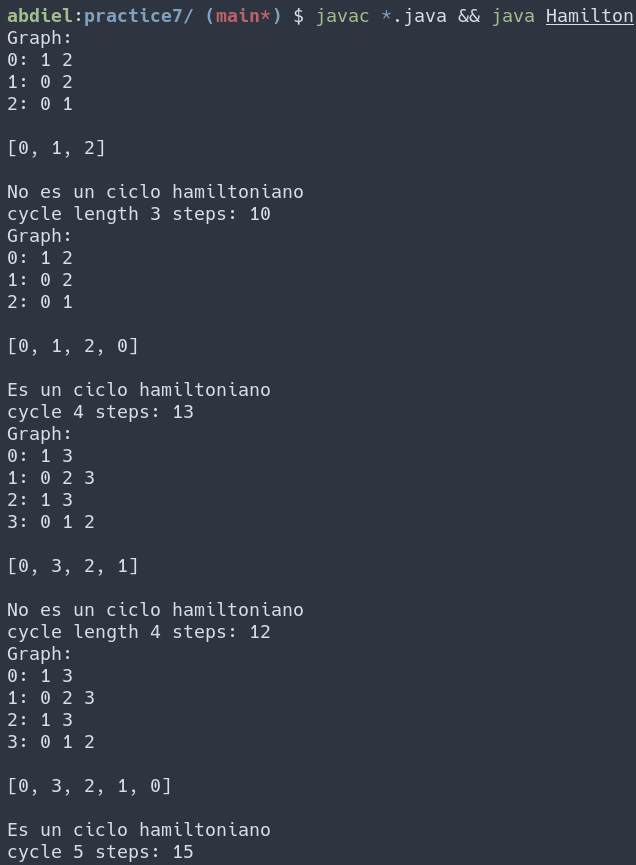
\includegraphics[width=0.4\textheight]{out_console_1.png}
        \caption{Esta es la compilación y ejecución del código en consola, donde nos muestra el grafo, el certificado, los pasos que tuvo al ejecutarse y si es un ciclo hamiltoniano, o no}
        \label{fig:my_label}
    \end{figure}
    \newpage
    
    \begin{figure}[h!]
        \centering
        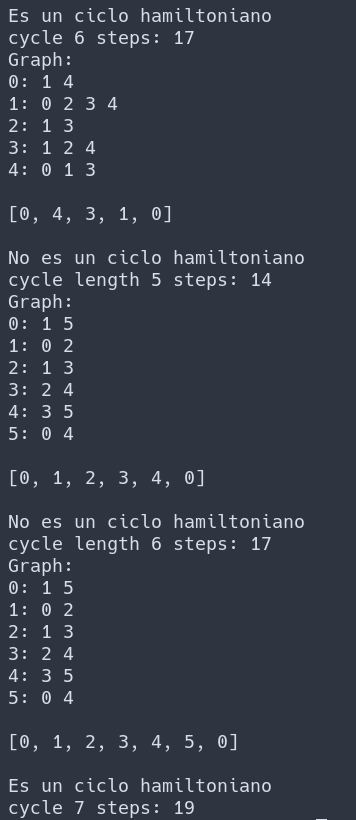
\includegraphics[width=0.3\textheight]{out_console_2.png}
        \caption{Esta es la compilación y ejecución del código en consola, donde nos muestra el grafo, el certificado, los pasos que tuvo al ejecutarse y si es un ciclo hamiltoniano, o no}
        \label{fig:my_label}
    \end{figure}
    \newpage
    \begin{table}[h!]
    \begin{tabular}{| c | c |}
            \hline
            n  & c   \\
    3 & 10 \\
    4 & 13 \\
    4 & 12 \\
    5 & 15 \\
    6 & 17 \\
    5 & 14 \\
    6 & 17 \\
    7 & 19\\
        \hline
    \end{tabular}
    \caption{Estos son los resultados de la ejecución del programa. En la primer columna, tenemos el tamaño del certificado con el cual se ejecutó, va del 3 al 7. En la segunda columna tenemos el valor del contador, que muestra el numero de instrucciones ejecutadas. Se observa como el crecimiento es constante}
    \end{table}
     \begin{figure}[h!]
            \centering
            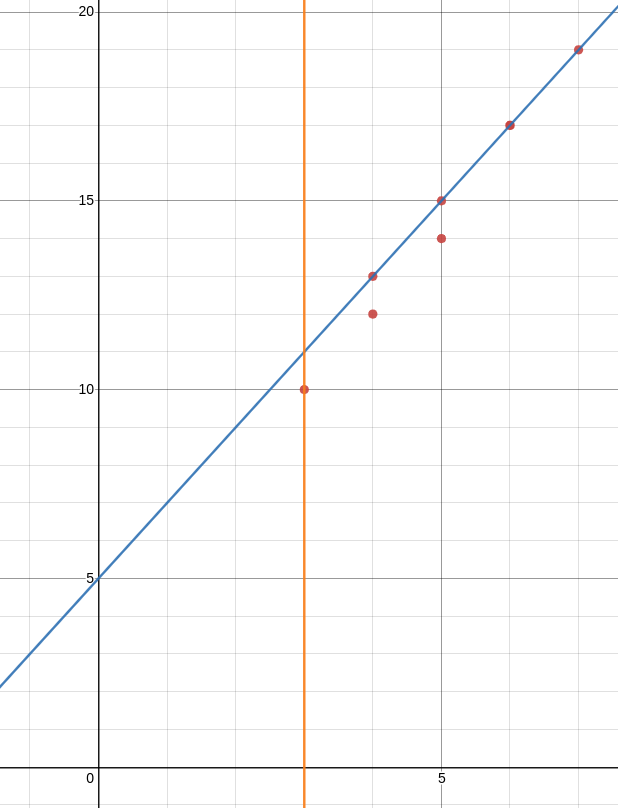
\includegraphics[width=0.4\textheight]{hamilton_graph.png}
            \caption{Esta es la gráfica que obtenemos de la tabla anterior. Los puntos son las coordenadas dadas por la tabla, la recta azul es la función $y=2x+5$ obtenida ajustando la ecuación de la recta y $n0$ está en el punto $(3,0)$}
            \label{fig:my_label}
        \end{figure}
    
        
        
    
\newpage
\section{Conclusiones}
    \begin{wrapfigure}{l}{0in}
        \centering
        
\includegraphics[scale=0.2]{abdiel.png}
    \end{wrapfigure}
    Enrique Abdiel Reyes Rodríguez:\\
    Lo más dificil a mi parecer fué el manejo de grafos, pensamos en usar C, pero nuestra habilidad con apuntadores no fué muy buena, por lo que optamos en usar Java.Logramos hacer nuestro Grafo usando un HashMap para evitar iterar de más en nuestra implementación. Se me hizo interesante el analisis de la verificación para concluir que es un problema NP, ya que muchas soluciones que observamos eran no tratables, siendo de orden exponencial.\\
    
    
    \begin{wrapfigure}{r}{0in}
        \centering
        
\includegraphics[scale=0.2]{diego.jpg}
    \end{wrapfigure}
    Juan Diego Chávez Hernández:\\
    Como práctica final pienso que juntar el tema de P vs NP fué una buena idea, sobretodo para comprender que tan viables son los problemas para computarse. Fué de mucha ayuda el comprender bien el problema, para pensar que era NP al inicio, ya que no logramos hallar soluciones que fueran polinómicas.\\
    
    \newpage
\section{Anexo}
    \subsection{Análisis a priori del algoritmo utilizado }
    Por medio del análisis por bloques de código vamos analizando el orden de complejidad de adentro hacia afuera. Empezamos por dentro del for, y vemos que todas sus instrucciones son constantes, el segundo if puede generar confusión, pero debemos recordar que $k$ tiende como máximo a el numero de vértices que tiene el grafo, siendo constante; por lo cual queda $O(n*k) = O(n)$. La instrucción del nivel superior también es constante, así que $O(n+1) = O(n)$.\\Vemos que para este caso, se tiene que $T(n) \in O(n)$\\
     \textbf{Pseudocódigo de la verificación de el ciclo hamiltoniano}
        \begin{verbatim}
function verificaHamilton(Grafo g,Certificado c)
   flag --------------------------O(1)
    for i = 0, i < c.length , i++ -----------------------------------------O(n*k)--O(n)
        if i+1 >= c.length && C[i]==C[0] && i== G.vertex.length----------O(1)
            flag = true -------------------------------------------O(1)-|
        else if !( map.vertex[C[i]].contains(C(i+1)) ) -----------O(k)
            flag = false-----------------------------------O(1)-|
            
    return flag
        \end{verbatim}\\
    Recordando que, la definición de NP menciona que para pertenecer a este, el certificado (en este caso, el camino que seguirá el grafo) puede ser verificado en tiempo polinómico. Nuestra verificación nos dió como resultado una complejidad de $O(n)$ por lo que concluimos que el Problema del Ciclo Hamiltoniano es \textbf{NP}. 
    \begin{figure}[h!]
        \centering
        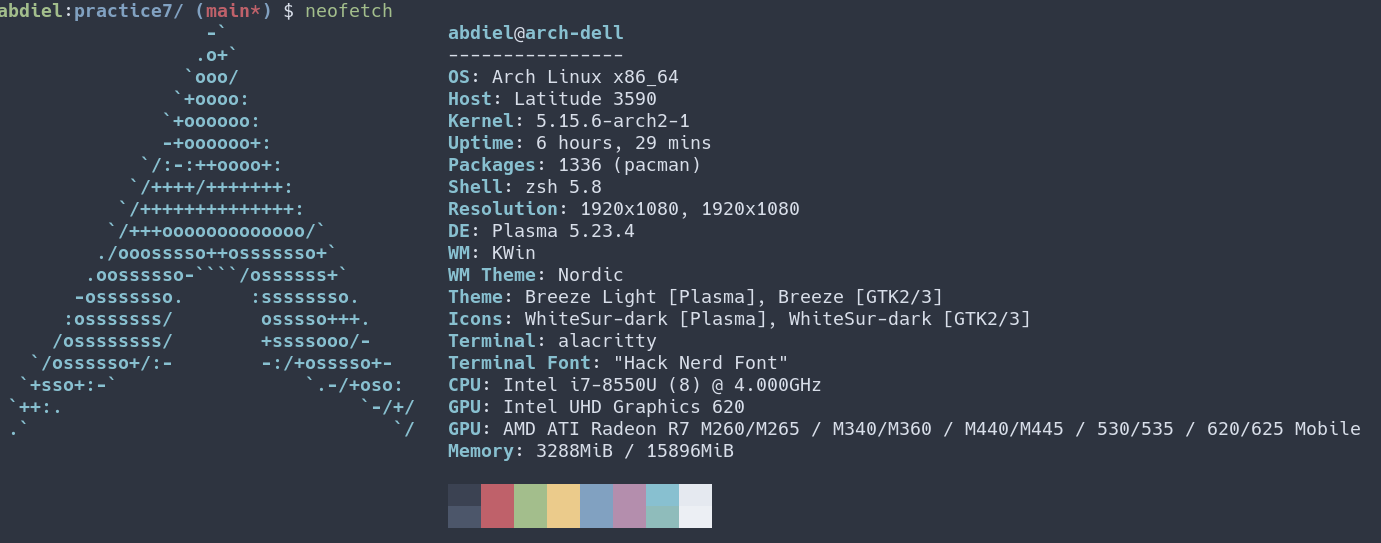
\includegraphics[width=1\textwidth]{specs.png}
        \caption{Estas son las especificaciones del equipo donde fueron ejecutados los experimentos}
        \label{fig:my_label}
    \end{figure}

    
   
\newpage    
        
\begin{thebibliography}{}
    
        \bibitem{1}Lasker, R. (2018, 21 enero). P ≟ NP - Rashid Lasker. Medium. Recuperado 17 de diciembre de 2021, de https://medium.com/@rashidlasker/p-np-an-introduction-to-computer-sciences-most-interesting-problem-47869a34601a
        \bibitem{2}Finding Hamiltonian Cycle in Polynomial Time. (s. f.). Science Alert. Recuperado 17 de diciembre de 2021, de https://scialert.net/fulltext/?doi=itj.2006.851.859
        \bibitem{3}GRAFOS. (s. f.). CCIA. Recuperado 17 de diciembre de 2021, de https://ccia.ugr.es/%7Ejfv/ed1/tedi/cdrom/docs/grafos.htm
        
    \end{thebibliography}

\end{document}